\documentclass[11pt]{article}
\renewcommand{\baselinestretch}{1.05}
\usepackage[spanish]{babel}
\usepackage[utf8]{inputenc}
\usepackage{lipsum}

\usepackage{amsmath,amsthm,verbatim,amssymb,amsfonts,amscd}
\usepackage{graphicx, wrapfig}
\usepackage{float}
\usepackage{caption, subcaption}
\usepackage{tkz-fct}
\usetikzlibrary{babel}
\usepackage{pgfplots}
\usepackage{enumitem}
\usepackage{multicol, vwcol}
\usepackage{listingsutf8}
\usepackage{color}
\usepackage{hyperref}
\usepackage{booktabs}


\usepackage[sorting=none]{biblatex}
\bibliography{bibliography.bib}

\hypersetup{
    bookmarks=true,         % show bookmarks bar?
    unicode=false,          % non-Latin characters in Acrobat’s bookmarks
    pdftoolbar=true,        % show Acrobat’s toolbar?
    pdfmenubar=true,        % show Acrobat’s menu?
    pdffitwindow=false,     % window fit to page when opened
    pdfstartview={FitH},    % fits the width of the page to the window
    pdftitle={Visión por computador - Trabajo final},    % title
    pdfauthor={Francisco Luque, Maria del Mar Ruiz},     % author
    pdfsubject={Visión por computador},   % subject of the document
    pdfnewwindow=true,      % links in new PDF window
    colorlinks=true,        % false: boxed links; true: colored links
    linkcolor=gray,          % color of internal links (change box color with linkbordercolor)
    citecolor=cyan,         % color of links to bibliography
    filecolor=magenta,      % color of file links
    urlcolor=blue           % color of external links
}

\setlength{\parindent}{0pt}
\topmargin0.0cm
\headheight0.0cm
\headsep0.0cm
\oddsidemargin0.0cm
\textheight23.0cm
\textwidth16.5cm
\footskip1.0cm
\theoremstyle{plain}

\newtheorem{theorem}{Teorema}
\newtheorem{corollary}{Corolario}
\newtheorem{lemma}{Lema}
\newtheorem{proposition}{Proposición}
\theoremstyle{definition}
\newtheorem{definition}{Definición}
\newtheorem{example}{Ejemplo}

\newcommand{\N}{\mathbb{N}}
\newcommand{\Z}{\mathbb{Z}}
\newcommand{\Q}{\mathbb{Q}}
\newcommand{\C}{\mathbb{C}}
\newcommand{\R}{\mathbb{R}}

\begin{document}

\begin{titlepage}
  \centering
  {\scshape\LARGE Universidad de Granada \par}
  \vspace{1cm}
  {\scshape\Large Visión por computación \par}
  \vspace{1.5cm}
  {\huge\bfseries Clasificación de imágenes usando CNNs \par}
  \vspace{2cm}
  {\Large\itshape Francisco Luque Sánchez \\
    María del Mar Ruiz Martín\par}
  \vspace{2cm}
  
\includegraphics[width=.3\textwidth]{logougr.png}\par\vspace{1cm}
  % Bottom of the page
  {\large \today\par}
\end{titlepage}

\newpage

\tableofcontents

\newpage

\section{Introducción}

En esta práctica se tratará el problema de la clasificación de objetos
en imágenes, utilizando concretamente redes neuronales convolucionales
(\textit{CNNs}). El problema que se abordará consiste en tratar de
distinguir perros de gatos utilizando estos modelos. Se comenzará con
un modelo simple, el cual se irá modificando para tratar de mejorar su
capacidad para clasificar.

\subsection{Conjunto de datos utilizado}

El conjunto de datos utilizado se ha generado utilizando las bases de
datos mostradas en \cite{db1, db2, db3}. Se han extraído todas las
imágenes de las mismas y etiquetado en dos clases (perros y gatos),
obteniéndose un conjunto total de unos 13000 gatos y 25000
perros. Dicho conjunto se ha dividido en dos subconjuntos, un conjunto
de entrenamiento (unos 25500 ejemplos) y uno de test (en torno a 12500
ejemplos), tratando de mantener la proporción de perros y gatos lo más
parecida posible en ambos conjuntos.\\

En cuanto al tamaño de las imágenes utilizado, se han redimensionado
todas ellas a un tamaño de $64 \times 64$ píxeles con codificación RGB
(es decir, se trabajará con imágenes de entrada de tamaño
$(64, 64, 3)$. Se utilizan imágenes de tan pequeño tamaño porque el
uso de imágenes de mayor tamaño provoca un aumento de tamaño muy
notable de la red neuronal utilizada, lo que se traduce en un aumento
del tiempo de cómputo muy considerable. Además, se comenzó haciendo
una prueba con imágenes de tamaño $128 \times 128$, y la diferencia en
los resultados obtenidos no era significativa. Finalmente, este
trabajo tiene la finalidad de estudiar las diferencias de capacidad de
clasificación de las redes neuronales convolucionales en función a su
estructura y parámetros, por lo que en principio no necesitamos crear
ejemplos muy potentes que permitan una clasificación muy precisa.
Se decide por tanto utilizar imágenes de este tamaño, aunque pueda
provocar que en fases finales del trabajo se pierda un poco de capacidad
de predicción al no utilizar imágenes de tamaño mayor.

\subsection{Aspectos de implementación}

Todo el código se ha desarrollado utilizando el \textit{framework}
TensorFlow \cite{tf}, que es una librería de código abierto
desarrollada por Google, orientada a la implementación de soluciones
utilizando inteligencia artificial. Esta librería permite la definición
de forma sencilla de estructuras de redes neuronales de varios tipos,
entre ellas redes neuronales convolucionales, que es el tipo de redes
en las que se centra el trabajo. Además, permite especificar los recursos
del equipo que se destinan a cómputo, dando gran flexibilidad al programador
a la hora de hacer los experimentos. El primer modelo desarrollado, en
particular, se ha hecho utilizando un tutorial de la documentación
del \textit{framework}, que se puede consultar en \cite{cnn-tutorial}.\\

El código se ha estructurado en 5 archivos distintos para cada modelo.
En el archivo \texttt{model.py} se establece la estructura de la red
neuronal. En los archivos \texttt{model\_train.py} y
\texttt{model\_test.py} se establece la ejecución de las operaciones
de entrenamiento y test.  En el archivo \texttt{input.py} se
implementan las funciones de lectura de imágenes desde
archivo. Finalmente, el archivo \texttt{predict\_image.py} permite que
se pase un nombre de imagen como argumento, y se utiliza el modelo
entrenado para predecir si en dicha imagen hay un perro o un gato.

\section{Modelos implementados}

\subsection{Model básico (\texttt{base\_model})}

Comenzamos describiendo el primer modelo implementado. Es el modelo
más simple de los estudiados. Pasamos a ver su estructura.

\subsubsection{Estructura de la red}

La primera de las redes se organiza de la siguiente manera. Recibe un
batch de 128 imágenes de tamaño $64 \times 64\times 3$. La primera
operación que realiza consiste en una capa de convolución que extrae
64 filtros para cada una de las imágenes. Después, tiene una capa de
pool que reduce el tamaño de las imágenes a la mitad, por lo que tras
esta capa se tiene un conjunto de imágenes de tamaño
$128 \times 32 \times 32 \times 64$. Tras esto, se redimensiona la
capa para que tenga una forma de $128 \times 65536$ características, y
se pasa dicho vector a una capa completamente conectada de tamaño
$65536 \times 348$.  Esta capa completamente conectada se conecta a
otra capa completamente conectada con dos neuronas, que nos darán la
probabilidad de que el elemento pertenezca a la clase gato (neurona 0)
o la clase perro (neurona 1). Las funciones de activación de todas las
capas es la función \textit{Relu}. El esquema de la misma es el siguiente:

\begin{figure}[H]
  \centering
  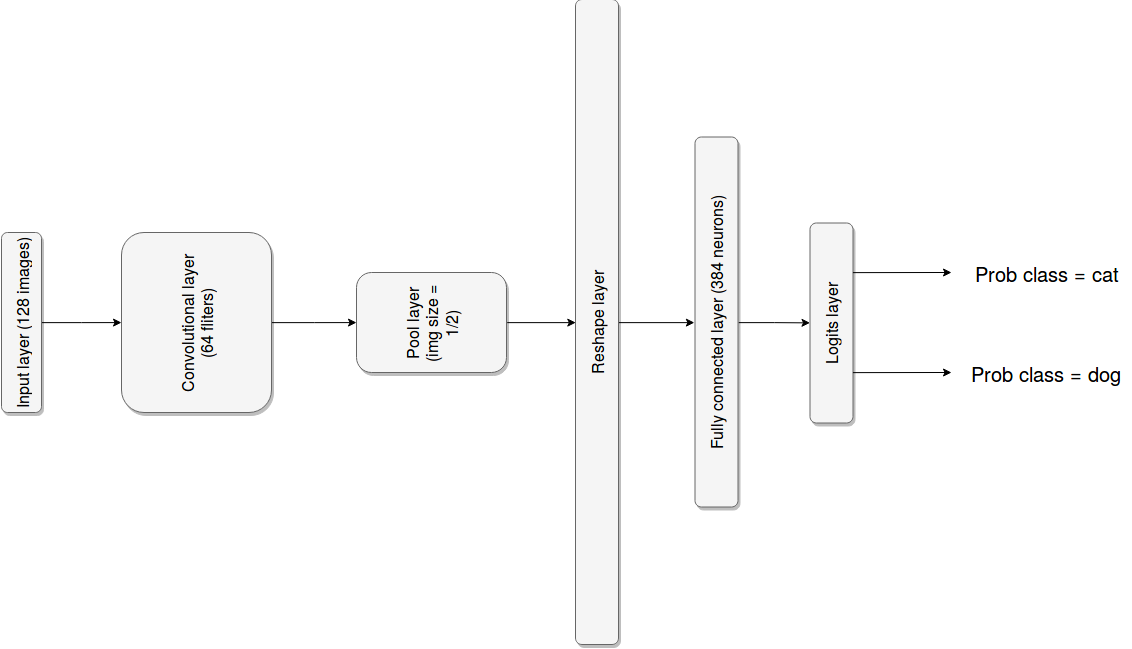
\includegraphics[width=.7\textwidth]{imgs/simple_model.png}  
  \caption{Esquema del modelo simple de red neuronal convolucional}
\end{figure}

\subsection{Aprendizaje de la red}

Una vez definida la estructura de la red, vamos a explicar ligeramente
el funcionamiento del aprendizaje de la misma. En cada etapa del aprendizaje,
se genera aleatoriamente del conjunto de imágenes de entrenamiento un subconjunto
de 128 ejemplos. 
\printbibliography

\end{document}